% !TeX root = ../main.tex
% LLD: Low Level Design

\chapter{详细设计与实现}

本章节在概要设计的基础之上,对本中文时间表达式信息抽取系统的详细设计给出具体解决方案并进行实现,主要包括各个模块的详细设计和逻辑实现。
本章节深入理解概率无关上下文语法的原理及其工作的上下文环境,设计实现各种识别和解析规则,完成本中文时间表达式信息抽取系统的编码实现。

\section{中文时间表达式识别模块的设计与实现}

\subsection{概述}

中文时间表达式的识别和解析都是以概率无关上下文语法为核心算法实现的。
对于中文时间表达式,涉及到两个比较关键的部分,一部分是对数字部分的识别,另一部分是对时间单元的识别,最后是有机的将这些识别规则组合到一起。
中文时间表达式识别模块的主要目的在于将识别到数字或时间单元的正则表达式映射到具体的实现类中,由实现类包含正则表达式规则与相应的关联文本。
可以用时序图的方式展现中文时间表达式识别的具体过程,如图~\ref{fig:recog_sequence}所示。

\begin{figure}[h]
    \centering
    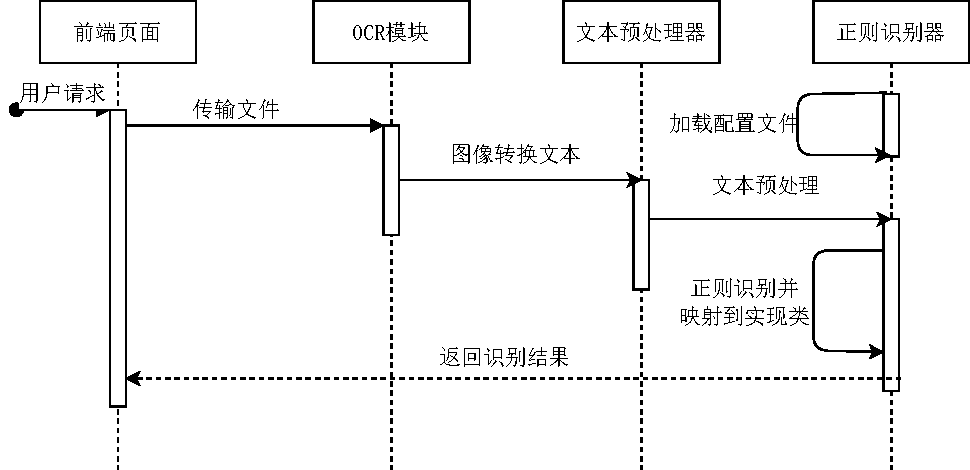
\includegraphics[width=1\textwidth]{recog_sequence.pdf}
    \caption{中文时间表达式识别时序图}
    \label{fig:recog_sequence}
\end{figure}

\begin{enumerate}
    \item[(1)] 首先正则识别器将在后台启动,加载用户配置文件,如果用户没有选择配置文件,将加载默认配置文件,配置文件主要包含正则识别的一系列终止符和非终止符。
    \item[(2)] 正则识别启动后,中文时间表达式识别模块将等待用户待识别数据的传入,如果用户传入的文件为PDF格式或图片格式,将先进入内部的OCR模块转化为一般文本。
    \item[(3)] OCR模块处理完后,将文本传输到文本预处理器,文本预处理器将作特殊符号以及简繁体等处理,使最终落库语料保持语言一致性,再交付到正则识别器。
    \item[(4)] 正则识别器根据预先配置的规则或者用户自定义的规则对文本进行识别,计算出目标实体在文本中的起止位置,并映射到实体类上。随后将识别结果返回前端并存储到数据库相应位置。
\end{enumerate}

下面几节将重点介绍正则识别器的相关设计与实现, 主要包含数值类型识别子模块和时间单元识别子模块。
% 概率无关上下文语法通常四元组的形式出现: (N,R,S,$\varSigma$)。
% 其中N代表的是非终止符号集合,$\varSigma$ 代表的是终止符号的集合。
% R代表的是一规则或者是产生式的结合,对于每一个产生式,其组成形式应该为 A $\rightarrow$ $\beta$[p],
% 其中A应该为一个非终止符,$\beta$是一个包含零个或多个符号的字符串,
% 字符串的形式应该为($\varSigma$ $\cup$ N),即非终结符与终结符的交集中产生的字符串。p则为一个介于0和1中间的数字,表示 P($\beta$|A)的概率。
% P($\beta$|A)可以理解为由终止符产生相应的表达式字符串的概率,即该产生式的概率。

\subsection{数值类型识别子模块的设计与实现}

\subsubsection{数值类型终止符定义的设计与实现}

\begin{table}[b]
    \centering
    \caption{部分数值类型终止符}
    \newcolumntype{Y}{>{\centering\arraybackslash}X}
    \begin{tabularx}{\linewidth}{YYYY}
        \toprule
        类名                                                                                                                 & 描述             & 蕴含字符                               & 对应数字                        \\
        \midrule
        CHINESE\_DIGITS                                                                                                      & 简体中文数字     & 〇,一,二,三,四,五,六,七,八,九 & 0,1,2,3,4,5,6,7,8,9    \\
        CHINESE\_DIGITS                                                                                               \_TRAD & 繁体中文数字     & 零,壹,贰,叁,肆,伍,陆,柒,捌,玖 & 0,1,2,3,4,5,6,7,8,9    \\
        CHINESE\_UNITS                                                                                                       & 简体中文数字单位 & 十,百,千,万,十万,百万             & $10^1,10^2,10^3,10^4,10^5,10^6$ \\
        CHINESE\_UNITS                                                                                                \_TRAD & 繁体中文数字单位 & 拾,佰,仟,萬,億                     & $10^1,10^2,10^3,10^4,10^8$      \\
        ARABIC\_DIGIT                                                                                                        & 阿拉伯数字       & 0,1,2,3,4,5,6,7,8,9           & 0,1,2,3,4, 5,6,7,8,9   \\
        MIXED\_SIGNS                                                                                                         & 正负符号         & 正,+,负,-                           & 1,1,-1,-1                    \\
        \bottomrule
    \end{tabularx}
    \label{tab:numeral_terminal}
\end{table}

数值类型终止符主要涉及到阿拉伯数字与中文数字的识别,考虑到实际的使用场景和目标群体,文字中并没有英文数字。

数值类型终止符主要通过继承TerminalSymbol类实现。每一个继承该类的子类都为相应的终止符。数值类型中比较核心的类有Comma,ArabicDigit,MixedSign,ChineseDigit,ChineseUnits。
数值类型终止符相关类的类图可见图~\ref{fig:numeral_terminal}。
如图中所示,每个终止符类中都包含一个RECOGNIZER字段,该字段对应RegexRecognizer类,此类为正则表达式的正则表达式解析器,可以将终止符定义的文字符号组织成正则表达式规则以解析所需要处理的自然语言文本。
以ArabicDigit类为例,其对应的文字符号将通过RegexRecognizer类的generate\_terminals方法组织成为 '$\left[ 0123456789 \right]$'的正则表达式形式,并通过Python语言底层的re模块,即正则表达式解析模块实例化为正则表达式类。
每个类对应的具体的自然语言文本可见表~\ref{tab:numeral_terminal}。

\begin{figure}[h]
    \centering
    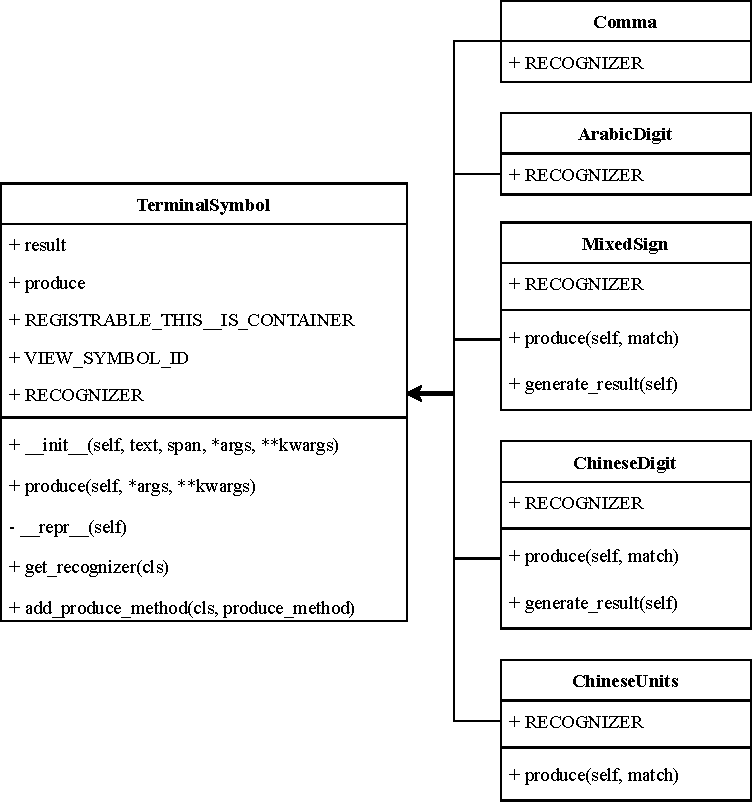
\includegraphics[width=0.8\textwidth]{numeral_terminal.pdf}
    \caption{数值类型终止符号类图}
    \label{fig:numeral_terminal}
\end{figure}

\subsubsection{数值类型非终止符的设计与实现}

\begin{table}[b]
    \centering
    \caption{部分数值类型非终止符及产生式}
    \newcolumntype{Y}{>{\centering\arraybackslash}X}
    \begin{tabularx}{\linewidth}{ccYc}
        \toprule
        类名                                              & 描述               & 部分产生式示例                                                                                             & 文本示例 \\
        \midrule
        \makecell*[c]{CHINESE                                                                                                                                                                          \\\_MIXED\_DIGITS\\\_AND\_UNITS}               & \makecell*[c]{携带单位的\\中文阿拉伯数\\字混合类型} & \textit{SelfRefSymbol}  \rightarrow MixedDigits + ChineseUnits;\textit{SelfRefSymbol} \rightarrow  ArabicUnsignedInteger + ChineseUnits & \makecell*[c]{3千4百\\八十六万} \\
        ARABIC\_DIGITS                                    & 阿拉伯数字         & \textit{SelfRefSymbol}   \rightarrow SelfRefSymbol + ArabicDigit;   \textit{A}   \rightarrow   ArabicDigit & 123045   \\
        \makecell*[c]{MIXED\_                                                                                                                                                                          \\DIGIT\_OOM}                                 & 混合型数字             & \textit{SelfRefSymbol}   \rightarrow MixedChineseArabicDigits + ChineseDigits;
        \textit{SelfRefSymbol}   \rightarrow MixedArabicChineseDigits + ArabicUnsignedInteger; \textit{SelfRefSymbol} \rightarrow  MixedChineseArabicDigits + ArabicUnsignedInteger;
        \textit{SelfRefSymbol} \rightarrow  MixedChineseArabicDigits;
        \textit{SelfRefSymbol} \rightarrow  MixedArabicChineseDigits;
        \textit{SelfRefSymbol} \rightarrow  ChineseDigits & \makecell*[c]{1二3                                                                                                                         \\四567}                                                                                                                                                                         \\
        \bottomrule
    \end{tabularx}
    \label{tab:numeral_nonterminal}
\end{table}

\begin{figure}[hbt]
    \centering
    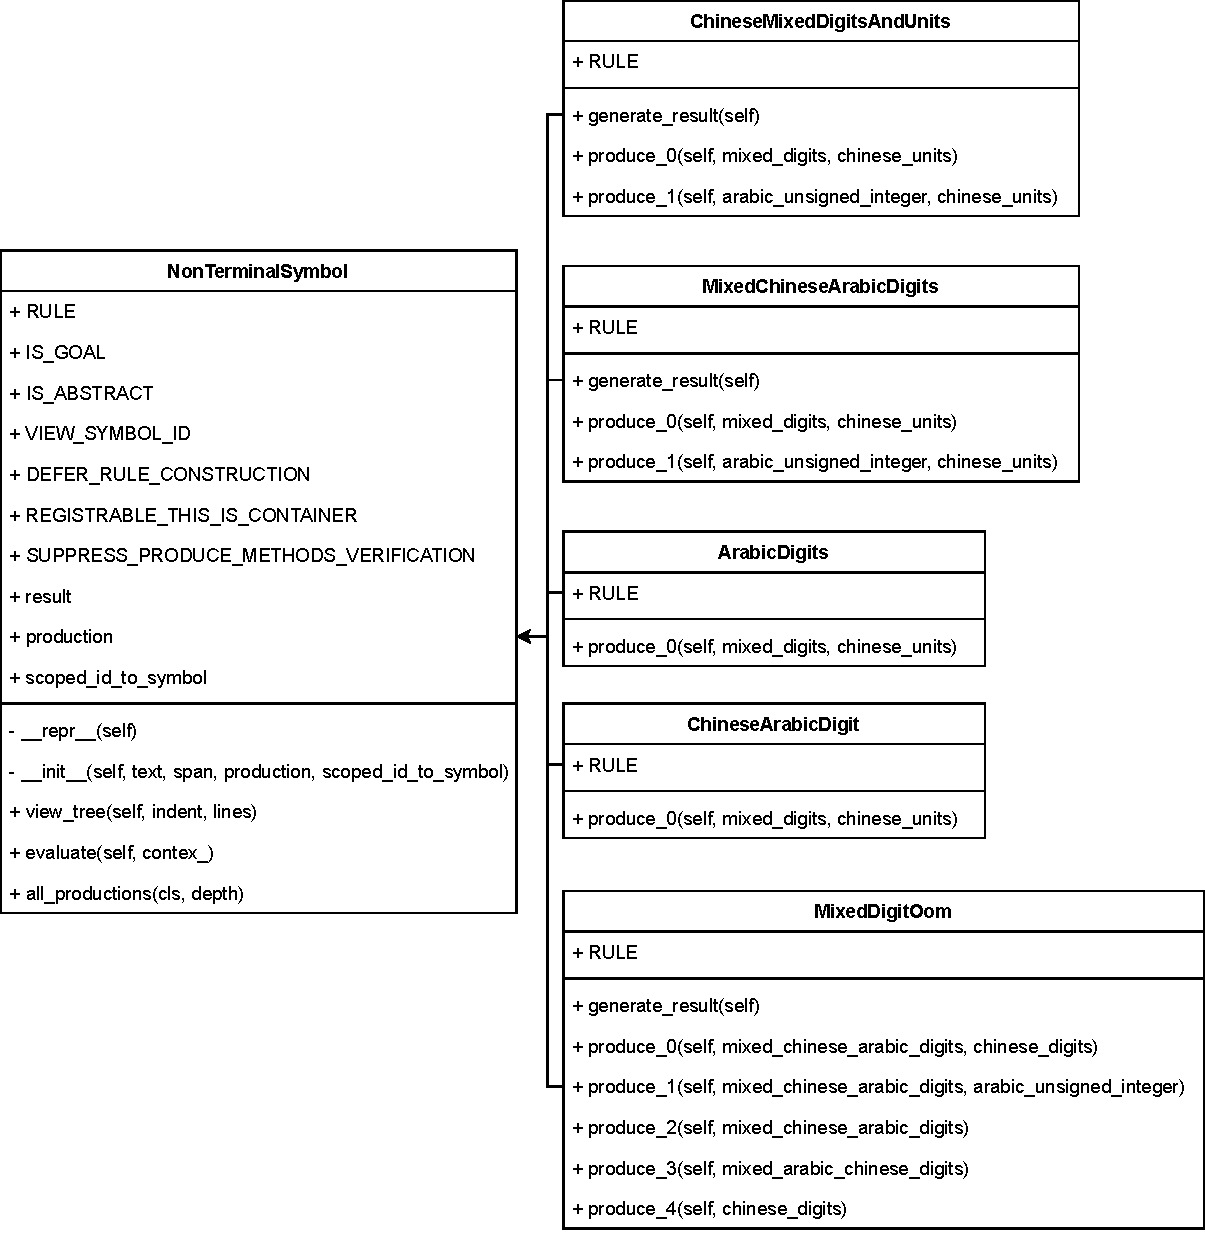
\includegraphics[width=1\textwidth]{numeral_nonterminal.pdf}
    \caption{部分数值类型非终止符号类图}
    \label{fig:numeral_nonterminal}
\end{figure}

数值类型非终止符的主要实现类需要继承NonTerminalSymbol,如图~\ref{fig:numeral_nonterminal}所示。
列举出来的一些NonTerminalSymbol的子类包括ChineseMixedDigitsAndUnits,MixedChineseArabicDigits,ArabicDigits,ChineseArabicDigit,MixedDigitOom等整数类型。
每个继承类的内部会包含RULE字段,该字段主要作用在于方便在解析的过程中收集与之相关的产生式。部分数值类型非终止符的产生式如表~\ref{tab:numeral_nonterminal}。

为了和非终止符,也就是TerminalSymbol类做出区分。NonTerminalSymbol中存在REGISTRABLE\_THIS\_IS\_CONTAINER字段,
将继承非终止符类的子类作为容器,装载一个或者多个产生式,不同的产生式将会按照
produce\_index\_in\_rule的形式,由专门的python元类处理,表示不同的产生式。如表~\ref{tab:numeral_nonterminal}中的MixedChineseArabicDigits类,因其关联到两个不同的产生式,所以其将分别
注入 produce\_0$\left(self,mixed\_digits,chinese\_units\right)$和produce\_1$\left(self,arabic\_unsigned\_integer,chinese\_units\right)$两个方法,方法中的参数为对应的产生式右侧的终止符或者非终止符。

数值类型非终止符起到的作用是集合或生成终止符或其他非终止符。和一般性的上下文无关语法不同的地方在于,在中文时间表达式识别过程中,如果能够匹配给定文本中的一部分规则,则其所匹配到的信息都具有一定的价值。
所以在组合规则的过程中会自然地形成类似于抽象语法树的结构,并在树中结点贮存相关的文本信息。
因此,每个继承NonTerminalSymbol的子类都需要显式地指定其是否为最终的起始符号,也意味着最终产生的概率无关上下文语法中将会有一个或多个起始符号,此时可以根据IS\_GOAL字段是否为真进行判断。
后续通过VIEW\_SYMBOL\_ID字段进行收集,再根据其真实符号的概率值进行判断和排序并输出结果。

\subsection{时间单元识别子模块的设计与实现}

\subsubsection{时间单元终止符的设计与实现}

\begin{table}[t]
    \centering
    \caption{部分时间单元终止符}
    \begin{tabular}{*{4}{c}}
        \toprule
        类名            & 描述                 & 蕴含字符                                 \\
        \midrule
        DUR\_UNIT\_HOUR & 以小时为单位的时间段 & 小时                                     \\
        QUANTIFER       & 量词                 & 个                                       \\
        UNIT\_WEEK      & 以周为单位的时间刻度 & $\left(\text{周|星期|礼拜}\right)$       \\
        UNIT\_THIS\_ADV & 副词,表示当前状态   & $\left(\text{这|今|本}\right)$           \\
        EVENT           & 特殊事件             & $\left(\text{中秋|国庆|辛亥革命}\right)$ \\
        \bottomrule
    \end{tabular}
    \label{tab:date_terminal}
\end{table}

\begin{figure}[h]
    \centering
    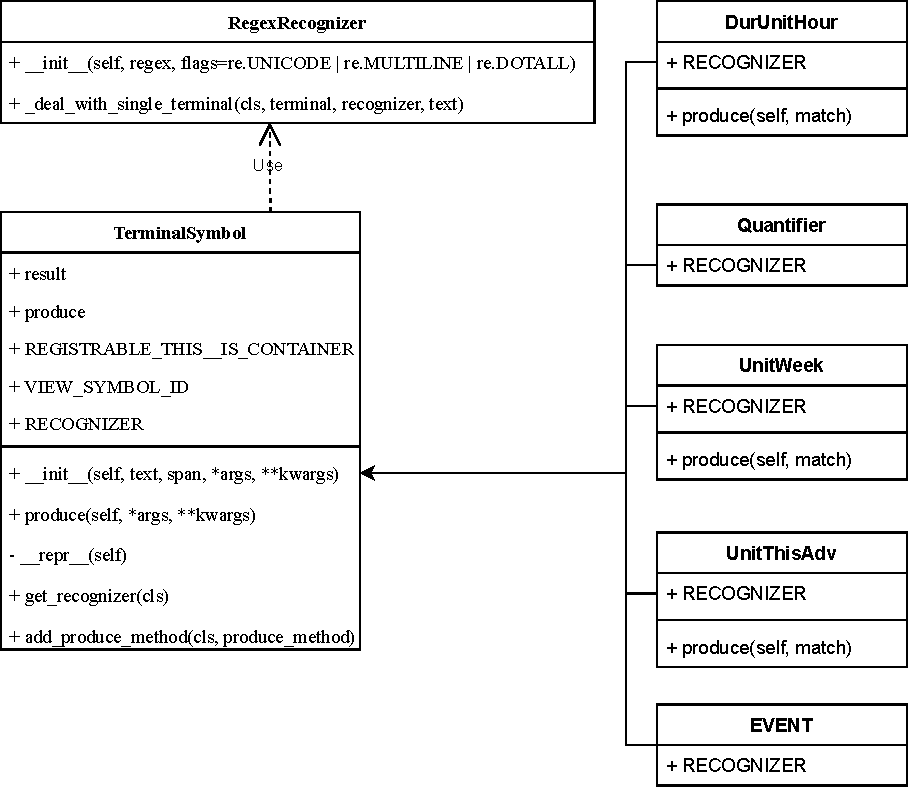
\includegraphics[width=0.75\textwidth]{date_terminal.pdf}
    \caption{部分时间单元终止符号类图}
    \label{fig:date_terminal}
\end{figure}

时间单元终止符的设计需要考虑到中文时间表达的多个时间维度修饰符,主要包括以下几种:
\begin{enumerate}
    \item[(1)] 时间刻度,如1998年,9月18日下午两点,周六晚七点等;
    \item[(2)] 时间段,如三天,24小时,一个钟头等;
    \item[(3)] 时间方位词,如前,后,去,下等;
    \item[(4)] 量词,如个,半等;
    \item[(5)] 特殊事件,如中秋节,国庆,辛亥革命。
\end{enumerate}

考虑到上述情况,针对不同的时间维度、时间范围分别设计对应的修饰符,表~\ref{tab:date_terminal}列举出部分时间单元终止符及其描述。


% TODO: 再加点内容
时间单元终止符的实现与数值类型终止符的实现大同小异,都需要继承TerminalSymbol类。其部分类图如~\ref{fig:date_terminal}所示。
其中比较典型的类有DurUnitHour,Quantifier,UnitWeek,UnitThisAdv,Event。

\begin{figure}[h]
    \centering
    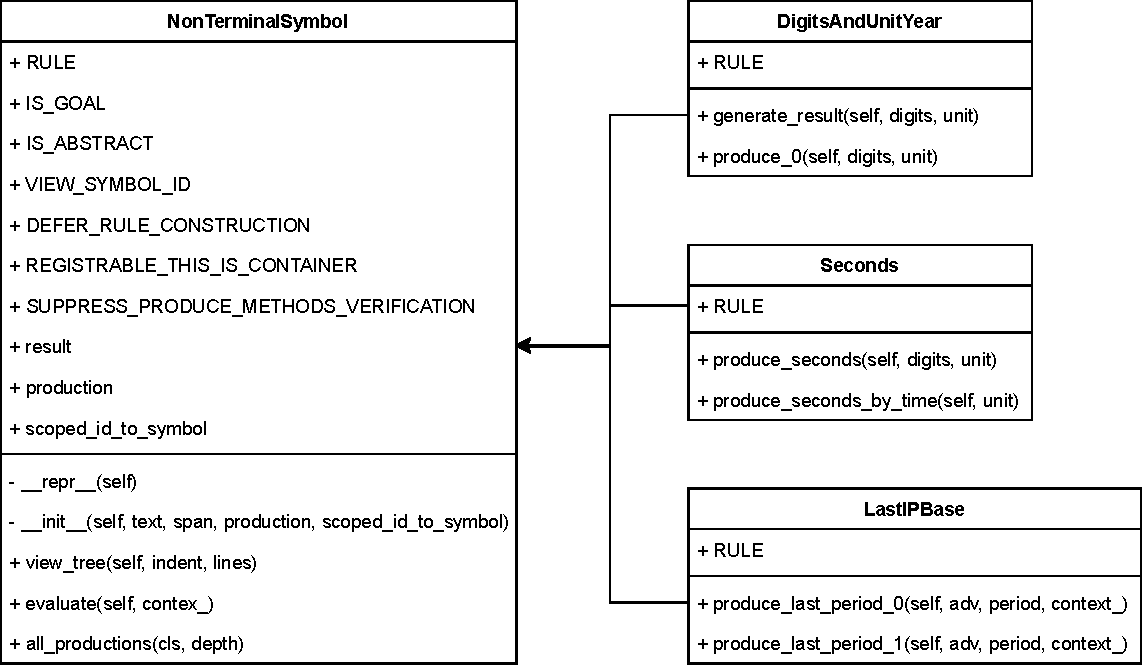
\includegraphics[width=1\textwidth]{date_nonterminal.pdf}
    \caption{部分时间单元非终止符号类图}
    \label{fig:date_nonterminal}
\end{figure}

\subsubsection{时间单元非终止符的设计与实现}

时间单元非终止符的具体实现除了要继承NonTerminalSymbol类,还依赖于数值类型的终止符与非终止符,部分实现类如下图~\ref{fig:date_nonterminal}所示。
时间单元非终止符的设计方式与时间单元终止符的设计思路一致,同样按照中文时间表达的多个时间维度(如小时,年月日等)、时间范围(一段时间)、关于时间的修饰符等设计规则并实现。

\section{中文时间表达式解析模块的设计与实现}

\begin{figure}[h]
    \centering
    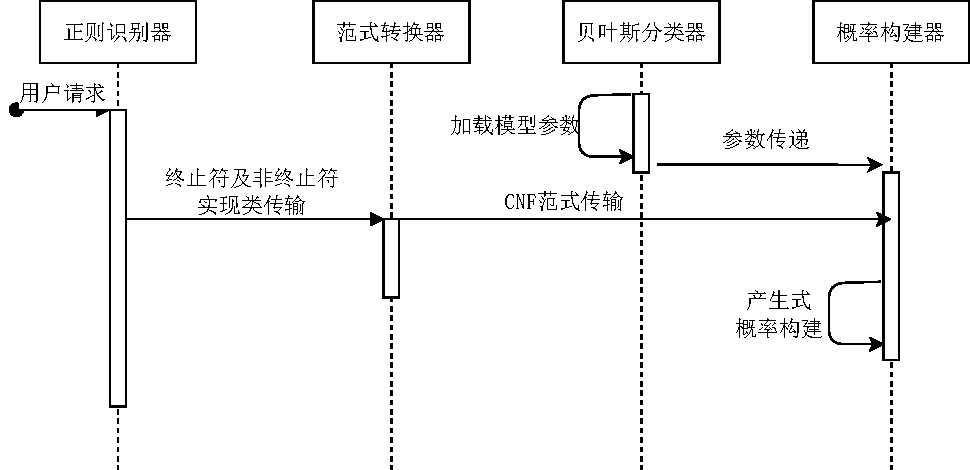
\includegraphics[width=1\textwidth]{resolve_preprocess_seq.pdf}
    \caption{预处理过程时序图}
    \label{fig:resolve_preprocess_seq}
\end{figure}

\subsection{预处理过程的设计与实现}

% TODO: 加点内容
前文给出了与时间表达式相关的终结符(terminal)和非终结符(non-terminals),终结
符在文本匹配中类似于正则表达式,用以确定时间表达式的区间(span)。非终结符则在最终对
时间表达式抽象成的语法树中充当非叶结点。由终结符和非终结符组成的产生式
(production)最终将被简化为 CNF(Chomsky norm function)。同时还需要向语料库中写入
语料,语料库中的每条数据应该以(文本,结果)的文本对的形式存储,语料库作为训练集以
求得每个产生式的似然。产生式的似然将参与求得语法树整体概率的计算。该过程可以用时序图表示,见图~\ref{fig:resolve_preprocess_seq}。



\subsection{分析树的构建过程的设计与实现}

\begin{figure}[h]
    \centering
    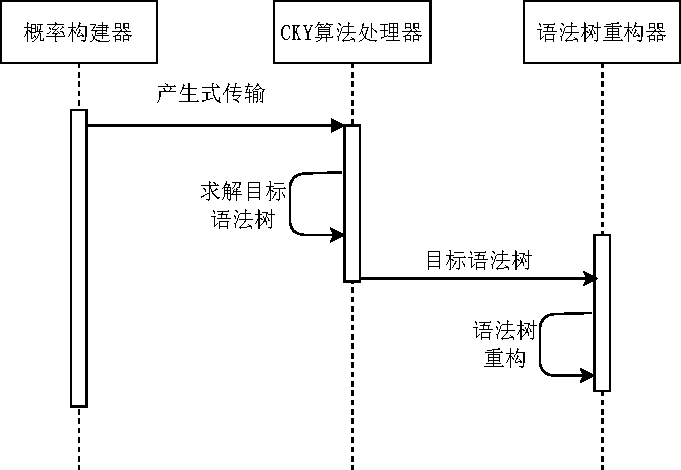
\includegraphics[width=0.8\textwidth]{resolve_treebuild_seq.pdf}
    \caption{分析树的构建过程时序图}
    \label{fig:tree_construction}
\end{figure}

分析树的构建过程如图~\ref{fig:tree_construction}所示,首先获取产生式的似然概率并简化CFG产生式为CNF,之后输入需要推理的文本(inference text)用以识别文本中的时间表达式,最后为识别出的时间表达式构建语法分析树。

同一时间表达式可能存在不同的解析方式,因此会产生不同的解析树,利用产生式的似然与CKY算法(Cocke–Younger–Kasami algorithm)推导最终可能产生的零个或多个CNF解析树。
分析树构建过程可见算法~\ref{algo:tree_construction}。
我们随后将CNF解析树还原为CFG解析树以还原分析树的初始状态,此时解析树中的非叶结点为上一小节中的非终结符,叶结点为终结符。图~\ref{algo:tree_construction}举例了一个时间表达式可能被解析成的一棵语法树。
左边分析树识别时间段(period)‘三日’,右边分析树识别日期(date)‘十月三日’,识别区间存在交集。分析树构建过程中,会调用树中各个结点的get\_result方法,将结点作为可加和性质的元素进行计算。
图~\ref{fig:tree_construction}中结点所含有的值即为分析树构建过程中的计算结果。

\begin{figure}[t]
    \centering
    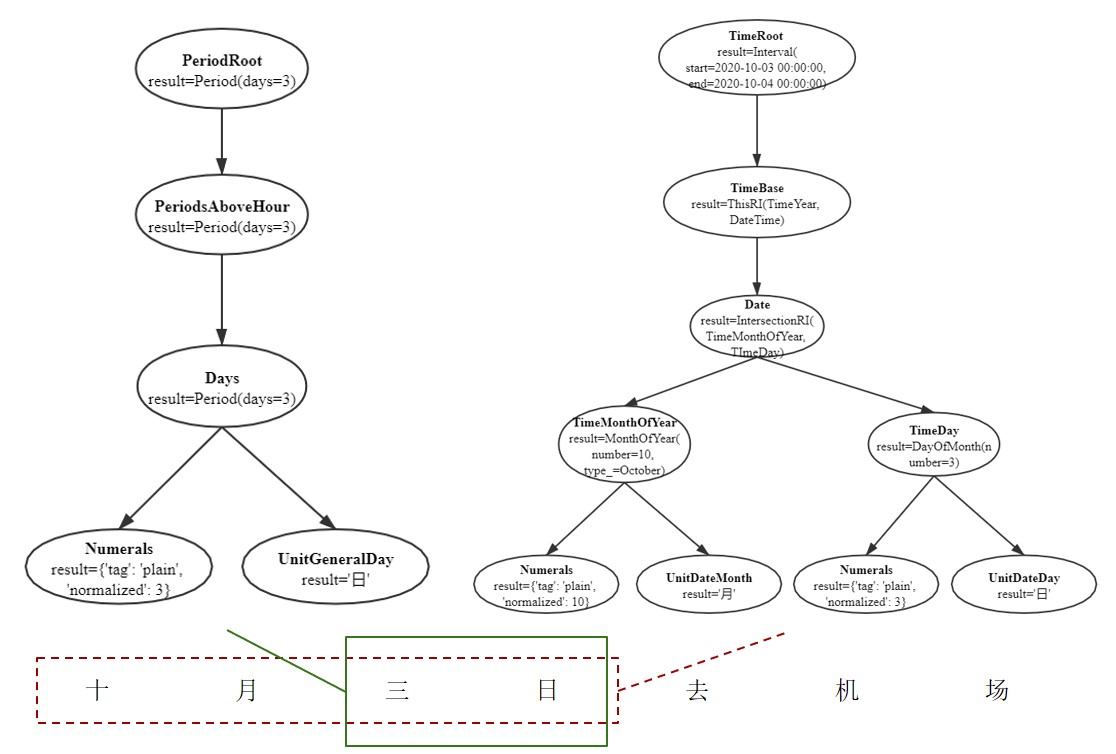
\includegraphics[width=1\textwidth]{example_1.pdf}
    \caption{时间表达式的语法冲突}
    \label{fig:example_1}
\end{figure}

\begin{algorithm}[htb]
    \SetAlgoLined
    \KwData{分析树构建算法}
    \KwResult{具有最大概率的一棵树以及该树的概率 }
    initialization\;
    \For{$j=0$; $j<length of input$; $j++$} {
        \ForAll{$A | A \rightarrow input[j] \in grammar$}{
            table[j - 1,j,A] \leftarrow P(A \rightarrow input[j])
        }
        \For{$i=j-2$; $i\ge0$; $i--$}{
            \For{$k=i+1$; $k<j$; $k++$}{
                \ForAll{$A | A \rightarrow BC \in grammar$ {\bf and} $table[i,k,B] \ge 0$ {\bf and} $table[k,j,c] \ge 0$}{
                    \If{table[i,j,A] \less P(A \rightarrow BC) \times table[i,k,B] \times table[k,j,c]}{
                        table[i,j,A] \leftarrow  P(A \rightarrow BC) \times table[i,k,B] \times table[k,j,c] \\
                        back[i,j,A] \rightarrow {k,B,C}
                    }
                }
            }
        }
    }
    \caption{分析树构建算法}
    \label{algo:tree_construction}
\end{algorithm}

\subsection{冲突消解的设计与实现}

\begin{figure}[b]
    \centering
    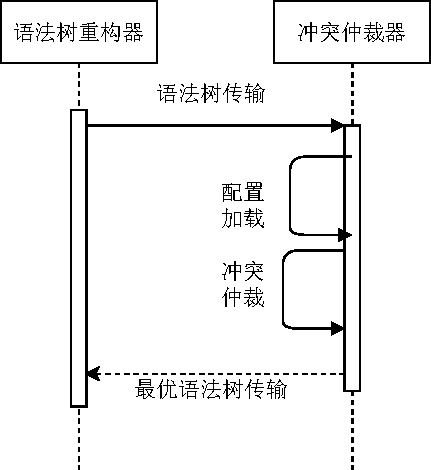
\includegraphics[width=0.55\textwidth]{resolve_conflict.pdf}
    \caption{冲突消解过程示意图}
    \label{fig:conflict_resolution}
\end{figure}

由分析树的构建过程可知,同一个时间表达式可能解析出多棵语法树,需要最终选择在总概率上为 top-k 的
k 棵语法树,即总体概率最大的 k 棵树。解析树的整体概率为树上所有产生式概率的乘积。冲突消解过程可见时序图~\ref{fig:conflict_resolution}。其过程可总结为: 

\begin{enumerate}
    \item[(1)] 冲突仲裁器加载用户配置,根据用户提供的上下文语境和设定的所需最优语法树的数量决定仲裁机制。如果用户没有配置选项,则加载默认配置文件。
    \item[(2)] 语法重构器将CNF语法树重构为CFG语法树后,将CFG语法树传输给冲突仲裁器负责仲裁。
    \item[(3)] 冲突仲裁器根据内置的冲突仲裁机制,选择最优的k棵语法树,将语法树保存到MongoDB中以唯一索引为标识符的位置上进行持久化,并将仲裁结果返回语法树重构器。
\end{enumerate}

\subsection{中文时间表达式的归一化}

在使用句法分析获得时间表达式的语法树后,还需要将整棵树归一化到一种具体的标注格式,归一化核心的数据结构有三:
\begin{enumerate}
    \item[(1)] Period(P):时间轴上的基本时间单位数量之和,如‘3 天’,‘2 个小时 30 分钟’;
    \item[(2)] Interval(I):时间轴上一段左闭右开的,能确定到年份(year)的区间,如‘2019 年’,‘2019 年 3 月’;
    \item[(3)] Repeat-interval(RI):时间轴上一段左闭右开的,不包括年份,表示在时间轴上具有重复性的一段区间,如‘3 月份’,‘5 点 20 分’。
\end{enumerate}

本中文时间表达式信息抽取系统以三种数据结构为核心,并用操作符集合(operator set)来表示时间表达式的语义,操作符本身也会继承NonTerminal类,并且作为分析树的根节点汇集树中所有结点的信息。
表~\ref{tab:operator} 中列举出部分典型操作符。在构建时间表达式分析树的过程中,其实已经将操作符与数据结构相结合,分析树构建完成后,
树的根结点会将操作符集合形成的嵌套表达式进行保存,直到需要将时间表达式转化为特定的结构化信息时才进行嵌套表达式的计算,以实现惰性计算(lazy evaluation)。
根结点的最终计算结果应该是以 ISO 格式描述的有起止时间的区间或类似格式的时间段。
如‘2019 年 3 月 2 日’,表达式最终计算的结果应该为‘Interval(start=2019-03-02T00:00:00,end=2019-03-03T00:00:00)’。

\begin{table}[h]
    \centering
    \caption{部分操作符语义}
    \newcolumntype{Y}{>{\centering\arraybackslash}X}
    \begin{tabularx}{\linewidth}{YYYY}
        \toprule
        操作符         & 函数                                  & 描述                                                     & 文本示例     \\
        \midrule
        SumP           & SumP(P,P) \rightarrow P              & 两个Period之和                                           & 两小时20分钟 \\
        IntersectionRI & IntersectionRI(RI,RI) \rightarrow RI & 两个Repeat-Interval之间的交集                            & 8月十五日    \\
        ThisRI         & ThisRI(I,RI) \rightarrow  I          & 根据Repeat-Interval确定年份                              & 8月十五日    \\
        BeforeIP       & BeforeIP(I,P) \rightarrow  I         & 将Interval向前移动Period的时间长度                       & 三天前       \\
        AfterRI        & AfterRI(I,RI) \rightarrow  I         & 重新定位Repeat-Interval                 在时间轴上的区间 & 3月25日以后  \\
        \bottomrule
    \end{tabularx}
    \label{tab:operator}
\end{table}

\section{时间信息抽取系统分析与展示模块}

对于训练好的中文时间表达式信息抽取系统,本地测试达到精度要求后,需要上线让用户使用,此时需要提供接口调用模型,企业内部对于用户提供了两种服务方式:SaaS 平台服务和线上 web 使用服务。

\subsection{自研Metis平台提供SaaS服务}

SaaS 服务应用于整个智能文档处理平台,综合了 OCR 识别、语料抽取、实体识别、中文时间表达式信息抽取和其他模型等,旨在让用户根据需求选择对应服务。SaaS 平台服务可以方便地实现模型的参数更新,还可以给用户更多的选择空间,
用户不仅可以上传和标注训练数据以更新模型参数并进行测试,还可以利用 微调选项 单独训练自己的特殊样本。在整个 SaaS 服务平台中,用户上传文档后通过 OCR 或直接文本读取进行
字符提取,然后使用中文表达式时间信息识别或解析模块处理用户数据,同时结合 UI 界面让用户方便地得到所需结果,极大地提高用户体验。

SaaS服务旨在通过网络请求获取结果,用户上传文件并调用接口发送请求后,服务器将接收数据并根据用户请求动作调用内部服务处理用户请求数据,最后返回用户需要的结果。
企业向外部提供SaaS服务的方式是使用企业内部自研的分布式服务体系框架Metis。
metis的设计思想是将具体的功能模块模块视为不可分的最小单元,可将这些单元组装成机器人并运行在企业平台上,机器人是将功能模块按照一定的执行流组装后的有向无环图,
本质上是一个有向无环图的执行流。
在下面所述步骤中,metis-mt指的是平台的任务调度器,负责调度机器人执行任务,worker则是工作线程, module指的是具体的功能模块。

\begin{enumerate}
    \item[(1)] 组装好机器人,加载配置文件并向metis-mt发送消息,将机器人注册到服务中心;
    \item[(2)] Metis-mt获取机器人的信息(dag),找到当下要执行的多个module;
    \item[(3)] Metis-mt向任务池发送所需的module运行配置,包含这个 module的 inputs、outputs、options 等,其中 inputs、outputs 的值是一段 short-id,指向真实数据的地址;
    \item[(4)] 相应的 worker从任务池中认领任务;
    \item[(5)] Worker在统一输入端口等待用户输入, 将解析用户输入并从一个地址信息转换为真实的内存数据,通过module的定义来调用;
    \item[(6)] Module按照配置处理用户输入, 待Module处理完后将结果以元组的形式传回worker;
    \item[(7)] Worker将结果数据反序列化并按照请求放到指定地点并通知metis-mt;
    \item[(8)] Metis-mt将处理数据返回用户;
    \item[(9)] 重复执行 (2)-(9)。
\end{enumerate}


因此,metis 可以采取模块化的方式进行配置,即模块调用需要配置数据传输方式以及调用模块的方式,之后按照上线打包的方式就可以在 web 端使用。

通过模块化的设计,将整个用户需求分成一系列步骤来处理,在每一步中都只用考虑对应的任务,这种模块化的方法将开发和应用分开,不仅可以方
便的进行模型开发,应用时只需要额外定义一个调用方法,便很简单方便地完成配置。其次,将任务以模块划分,将系统的功能相独立,可以实现系统的高拓展
性及可维护性。

Metis 中,包括输入模块、输出模块在内的所有流程都是模块化的,每个模块都有对应的 inputs、outputs 和 options。文档分类模块旨在判断文档类型属于电子版或图片版,判断逻辑影响输出 outputs,
不同的输出会分别作为 PDF 页面分割模块和 OCR 识别模块的输入 inputs,而PDF 分割页面模块中的循环逻辑则由模块内 options 决定。整个流程是线性执行的,而每个模块的输出都可以连接到结果展示模块,以方便用户预览和下载数据。

% 将若干测试数据输入对应的UI测试页面,可以得到相应的结果,其结果如图~\ref{fig:web_result}所示。其中OPERATORROOT即为上文中提到的操纵符作为根节点识别到的结果,TIMEROOT则是文本作为准确的时间刻度识别到的文本。

% \begin{figure}[h]
%     \centering
%     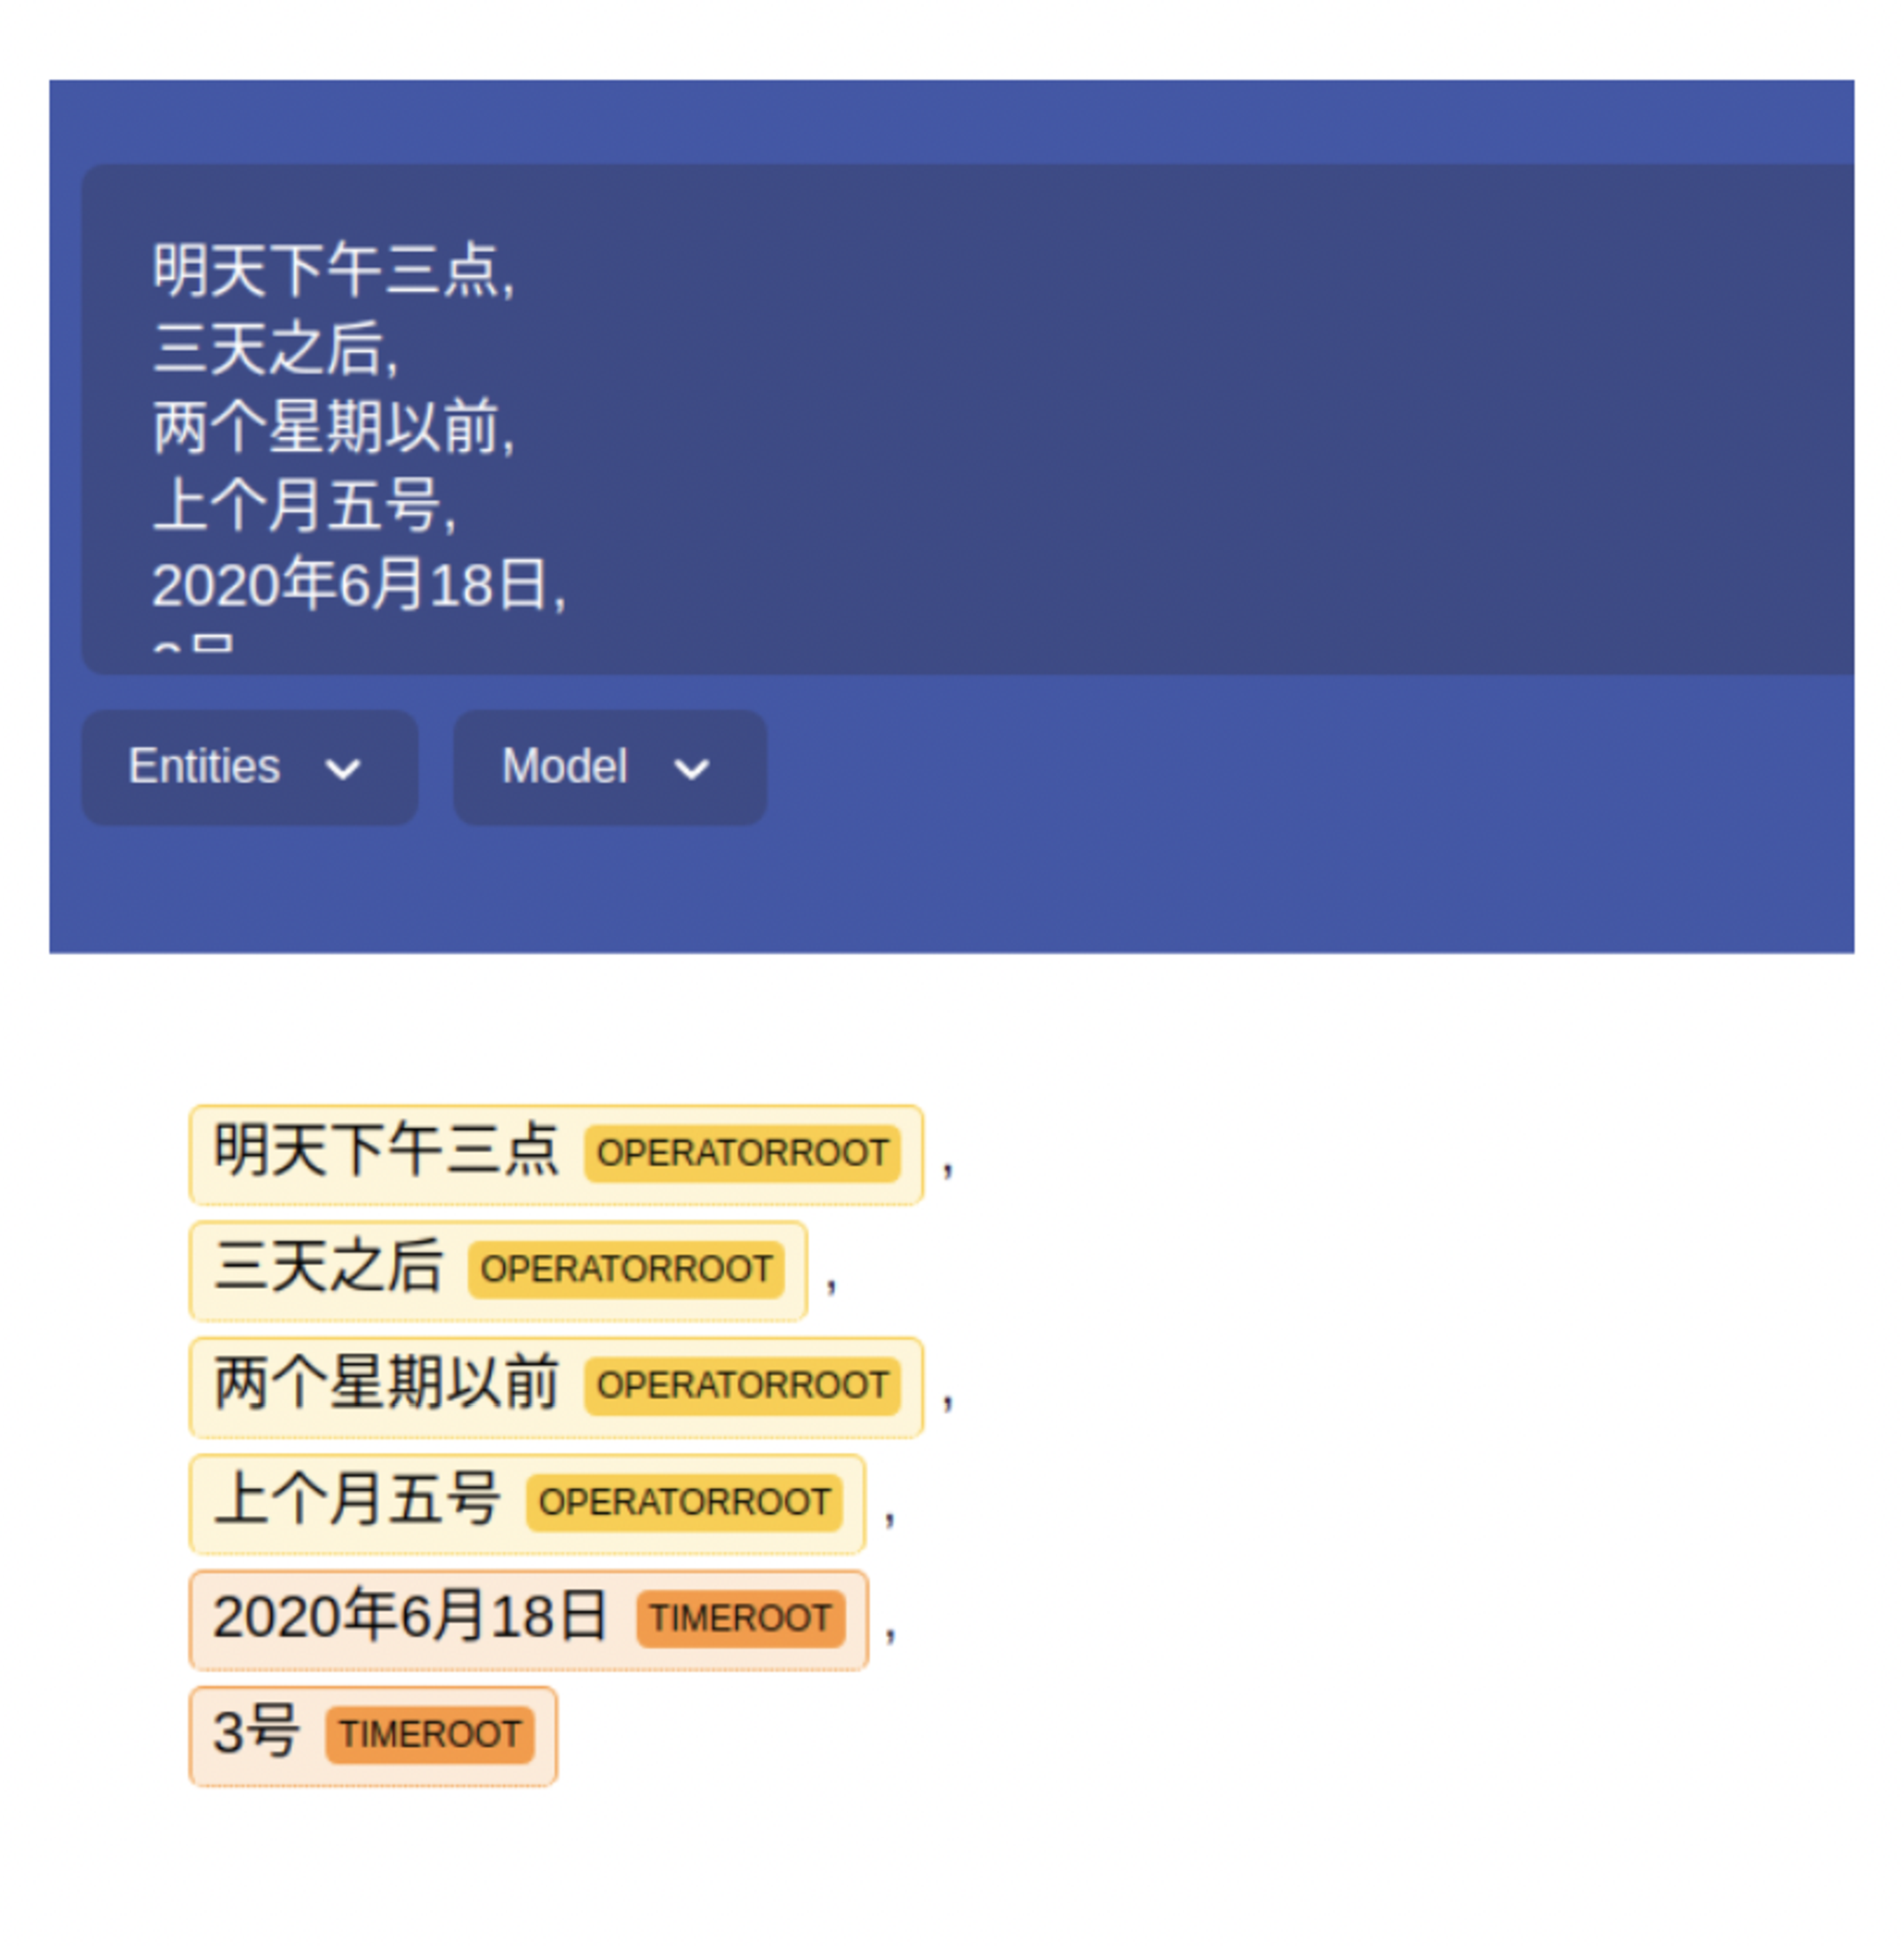
\includegraphics[width=0.75\textwidth]{web_result.pdf}
%     \caption{UI测试页面}
%     \label{fig:web_result}
% \end{figure}

\section{时间信息抽取系统分析结果与语料存取模块}

% TODO: 扩写该小节
时间信息抽取系统分析结果与语料存取模块主要是将用户传入的数据以及解析后的结果记录在MongoDB中,用户传入的数据首先会在内存中转换为Json形式,再通过序列化的方式传入MongoDB中进行持久化操作。
当前时间信息抽取系统分析结果与语料存取模块包含将Json文件导入数据库、数据完整性校验、数据分表存储、数据表索引加速等功能。其时序图如图~\ref{fig:mongo_seq}。


\begin{figure}[h]
    \centering
    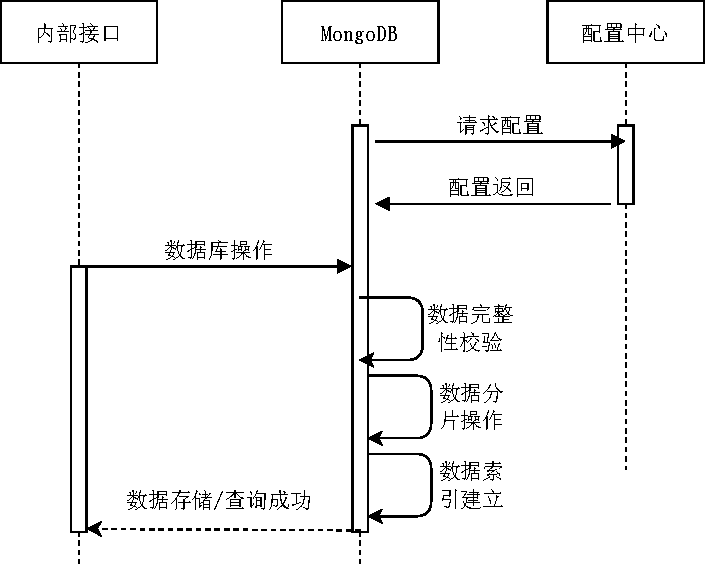
\includegraphics[width=0.8\textwidth]{mongo_seq.pdf}
    \caption{时间信息抽取系统分析结果与语料存取模块时序图}
    \label{fig:mongo_seq}
\end{figure}

\begin{enumerate}
    \item[(1)] 首先后端服务向配置中心获取相应的配置文件,根据配置文件中的配置连接MongoDB;
    \item[(2)] 如之前所述,中文时间表达式识别模块会将与正则规则对齐的文本信息持久化,同时中文时间表达式解析模块会将最终的解析结果进行持久化,此时通过内部接口调用MongoDB服务;
    \item[(3)] MongDB服务根据配置中的数据完整性校验选项,对内部接口传输的数据经i选哪个完整性校验,并根据唯一标识符将文件路由到相应分区存储,并更新数据索引;
    \item[(4)] 外部接口调用成功,将完成日志或查询记录返回给内部接口,关闭数据库连接。
\end{enumerate}


\section{本章小结}

% TODO: 加点,譬如最终实现以及提供的服务
本章主要介绍了基于概率无关上下文语法的中文时间表达式信息抽取系统的详细设计和实现,
首先从整体描述了系统的架构和各个模块的结构,包括中文时间表达式识别模块的设计与实现、中文时间表达式识别模块的设计与实现、
时间信息抽取系统分析与展示模块的设计与实现、时间信息抽取系统分析结果与语料存储模块的设计与实现。
部分模块还给出了相关流程图和类图详细设计。
